\documentclass{article}

% if you need to pass options to natbib, use, e.g.:
% \PassOptionsToPackage{numbers, compress}{natbib}
% before loading nips_2017
%
% to avoid loading the natbib package, add option nonatbib:
% \usepackage[nonatbib]{nips_2017}

\usepackage[final]{nips_2017}


\usepackage[utf8]{inputenc} % allow utf-8 input
\usepackage[T1]{fontenc}    % use 8-bit T1 fonts
\usepackage{hyperref}       % hyperlinks
\usepackage{url}            % simple URL typesetting
\usepackage{booktabs}       % professional-quality tables
\usepackage{amsfonts}       % blackboard math symbols
\usepackage{nicefrac}       % compact symbols for 1/2, etc.
\usepackage{microtype}      % microtypography
\usepackage{graphicx}


% Choose a title for your submission
\title{Tackling Story Cloze Test with Wrong Ending Generation}


\author{Pascal Wiesmann \qquad Stefano Woerner \qquad Sandar Felicity Lim}
%\graphicspath{{fig/}}
\begin{document}
% \nipsfinalcopy is no longer used

\maketitle

% We do not requrire you to write an abstract. Still, if you feel like it, please do so.
%\begin{abstract}
%\end{abstract}

Feel free to add more sections but those listed here are strongly recommended.
\section{Introduction}
You can keep this short. Ideally you introduce the task already in a way that highlights the difficulties  your method will tackle.

\section{Methodology}
\subsection{Generating wrong endings with WordNet}
Wrong endings were generated for each story to better train our classifier. Naive way would be to randomize the correct endings of each story. However, doing so would obviously change the main charecter or main point of the story. Therefore, we needed to generate endings that are wrong but still preserves narrative structure. Negation of the fifth sentence was a promising way to achieve that end. i.e. The resulting sentence would be contain at least one of the charecters of the story. The resulting sentence would still be generally realisitic, except that it would not create a meaningful story as an addition to the previous four sentences.


Negation can be challenging for complex sentence structures because we would have to decide which part of the sentence to negate. For example, the sentence: "
Kelly quickly went home." There are two possibilities of negation: "Kelly slowly went home" or "Kelly did not quickly go home". If we do not keep track the number of negations in the sentence, the result would be wrong: "Kelly did not slowly go home", which is not the negation of the original sentence. Hence, our approach, as shown in  Figure \ref{Figure:wrong}, was to first negate the adjectives and adverbs, and in their absence, negate the verbs, all the while keeping count of number of negations in the generated sentence.

\begin{figure}
  \centering
  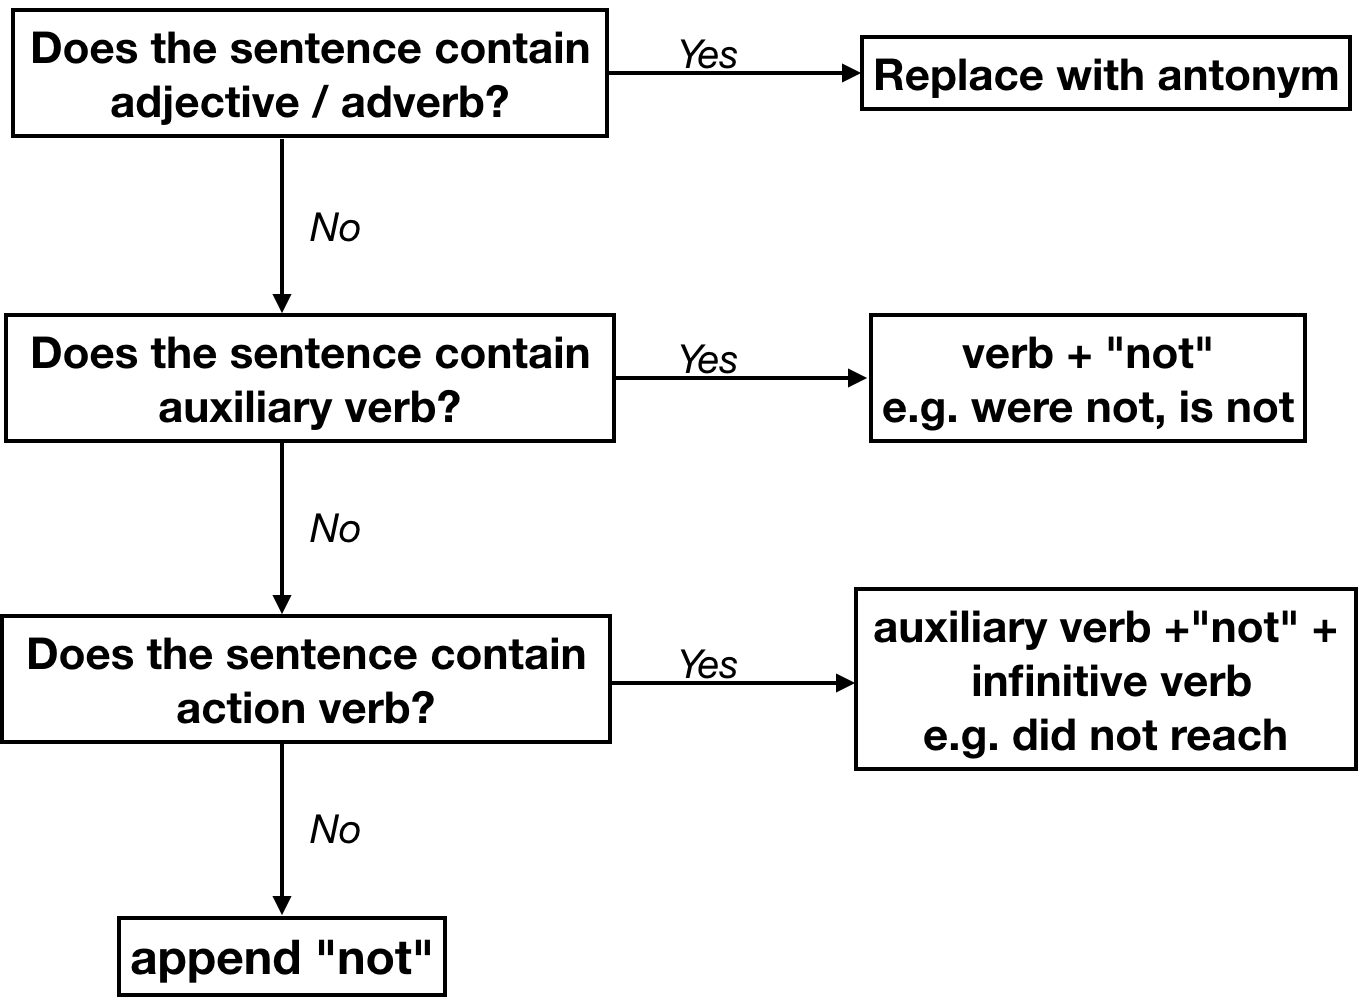
\includegraphics[width=0.7 \linewidth]{fig/wrong.PNG}
  \caption{Our apporach to generate wrong endings}
  \label{Figure:wrong}
\end{figure}


A few examples of our successful sentence generations are shown in Table \ref{Tab:works}

\begin{table}[h]\footnotesize
  \centering

  \begin{tabular}{ p{6cm} p{3cm} p{3cm} }
    \toprule
    Context & Right Ending & Wrong Ending \\
    \midrule
    The family was tired of not hearing when someone knocked on their door. They installed a doorbell on their front door. It would ring a pleasant tune when someone came to see them. They never missed houseguests anymore.  & The family wished they'd gotten the doorbell earlier! & The family wished they'd gotten the doorbell late! \\
    \hline
    Tim was hiking up a mountain with friends. He wasn't paying attention and lost his footing. Tim tumbled down down for a few yards. He was severely hurt. & Tim's friends had to call for help and carry him. & Tim 's friends did not have to call for help and carry him . \\
    \hline
    Laura found a jar of candy in her mom's kitchen. Laura ate all of the candy. She got really sick. Laura's mom discovered why Laura was sick. & Her mom felt bad for her so she didn't punish her for eating it all. & Her mom felt good for her so she didn't punish her for eating it all.\\
    \bottomrule
  \end{tabular}
  \label{Tab:works}
  \caption{Generated wrong endings that works}
\end{table}

\subsubsection{Limitations}
There are two main limitations of our model to generate wrong endings. First, is that our antonym replacement may not be sensible at times \citep{wordnet}. Table \ref{Tab:strange} shows a few examples of sentences are grammatically wrong or not sensible.

\begin{table}[h]\footnotesize
  \centering
  \begin{tabular}{ p{6cm} p{3cm} p{3cm} }
    \toprule
    Context & Right Ending & Wrong Ending \\
    \midrule
    Gina's brother Jay had been out of the house. Now he was back. He'd fought their father. Their dad was a foot taller and 50 pounds bigger. & Gina no longer felt safe with him around. & Gina yes longer felt safe with him around.\\
    \hline
    Matthew grew up with a dad that pushed him in sports.,He thought he would grow up to be an athlete. Once he grew up he realized he wanted to do other things. His dad was very angry. & Their relationship got bad and they no longer talked. & Their relationship got good and they no longer talked. \\
  \bottomrule

  \end{tabular}
  \label{Tab:strange}
  \caption{Generated wrong endings that are not sensible. In the first story, the phrase "yes longer" does not exists in English. In the second story, the sentence is connected by "and" but negation was only applied once.}
\end{table}

Second is that our generated wrong endings may have high occurance of the word "not" as our model was designed to insert "not" in the absence of antonyms. This would affect our classifier performance negatively.

\subsection{Generating wrong endings with seq2seq}
We adapted the neural machine translation tutorial on Tensorflow which made use of seq2seq models \cite{tfseq2seq}. Sequence2sequence model consists of two RNNs: encoder and decoder, which reads the  input sequence to infer semantic summary and generates output sequence respectively. Our method starts with training the model on true endings of the train dataset. Then we did a post-training on 80\% of the wrong endings of validation set. We included validation set in our training model because doing so further impoves the ability of our model to generate wrong endings.


\subsubsection{Limitations}


\section{Model: Classifier}

Figure \ref{Figure:model} shows the architecture of our model. This is similar to the approach by Burgert et al. except for a few differences \cite{top4}. Our model involves two Long Short-Term Memory (LSTM) units to compute the feature representation of each sentence \citep{lstm}, instead of one Bidirectional Recurrent Neural Network (BiLSTM).

Firstly, we looked up the word embedding of each word in vector space for each sentence. The embeddings from the first four sentences were then passed on to the first LSTM which summarises the story in numbers. Likewise, the last sentence was passed on to the second LSTM. The results of two LSTMs are then concatenated as a string and passed on to a dense layer. The classifier trains on where the ending is relevant to the story or not.

\begin{figure}
  \centering
  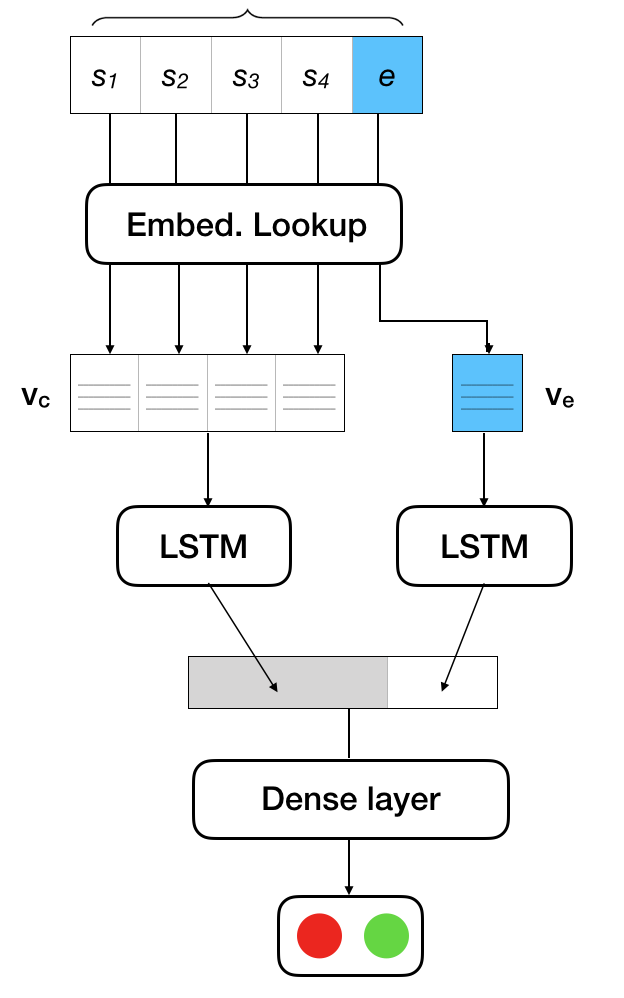
\includegraphics[width=0.5 \linewidth]{fig/ourmodel.PNG}
  \caption{Our classifier}
  \label{Figure:model}
\end{figure}

\section{Training}
What is your objective? How do you optimize it?

\section{Experiments}
This {\bf must} at least include the accuracy of your method on the validation set.

\subsection{Results}
\begin{table}[h]
  \centering
  \begin{tabular}{ c c c c}
    \toprule
    Approach &  \multicolumn{2}{c}{Validation} & Test \\
     &  Dev & Full &  \\
    \midrule
    Happy & 0.616 & 0.590& 0.602\\
    Happy & 0.616 & 0.590& 0.602\\
    Happy & 0.616 & 0.590& 0.602\\
    Happy & 0.616 & 0.590& 0.602\\

    \bottomrule
  \end{tabular}
  \label{Tab:results}
  \caption{System accuracies on the Story Cloze datasets. }
\end{table}

\section{Conclusion}
You can keep this short, too.



\bibliographystyle{unsrt}
\bibliography{resources.bib}

\end{document}
